\chapter{Finite Difference Method}
In this chapter, we will discuss the finite difference method which is one of numerical methods for solving PDEs. Before finding the forward, backward and central difference formulas, we will briefly describe Taylor's theorem in one variable as follows:
%\begin{Theorem}[(Taylor's theorem)]{}
%	Let $f$ is continuous differentiable up to $n^{\text{th}}$ order and $f$ has $(n+1)^{\text{th}}$ derivative in the neighborhood of $a$. Then
%	$$f(x) = f(a) + (x - a)f^{'}(a) +   \dfrac{(x - a)^{2}}{2!}f^{''}(a)+\dots+ \dfrac{(x - a)^{n}}{n!}f^{(n)}(a) +R_{n}(x), $$
%	where
%	$$ R_{n}(x) =  \dfrac{(x - a)^{n+1}}{(n+1)!}f^{(n+1)}(c),$$
%	and $c$ is some point between $a$ and $x$. 	
%\end{Theorem}
\begin{Theorem}[{\cite[pp.10-11]{burden2011numerical}}(Taylor's theorem)]{}
	Suppose $f \in C^{n}[a, b]$, that $f^{(n+1)}$ exists on $[a, b]$, and $x_{0} \in [a, b]$. For every $x \in [a, b]$, there exists a number $\xi$ between $x_{0}$ and $x$ such that
	$$f(x) = P_{n}(x) + R_{n}(x),$$
	where 
	\begin{align*}
	P_{n}(x) & = f(x_{0}) + f^{'}(x_{0})(x - x_{0}) +   \dfrac{f^{''}(x_{0})}{2!}(x - x_{0})^{2}+\dots+ \dfrac{f^{(n)}(x_{0})}{n!}(x - x_{0})^{n},
%	\\
%	& =\sum_{k=0}^{n}\dfrac{f^{(k)}(x_{0})}{k!}(x - x_{0})^{k}	
    \end{align*}
	and
	$$ R_{n}(x) =  \dfrac{f^{(n+1)}(\xi)}{(n+1)!}(x - x_{0})^{n+1}.$$
	Here $P_{n}(x)$ is called the $n\text{th}$ Taylor polynomial for $f$ about $x_{0}$, and $R_{n}(x)$ is called the truncation error associated with $P_{n}(x)$.
\end{Theorem}

\section{First order forward difference}
\subsection*{In one dimension}
Let $\hspace{5cm} u: \mathbb{R} \longrightarrow \mathbb{R}$
\par
$ \hspace{5.8cm} x \longmapsto u(x)$
\\ 
be one dimensional function.
\\
The discretization of the interval $[a, b]$ into $N$ points is given as
	\begin{center}
		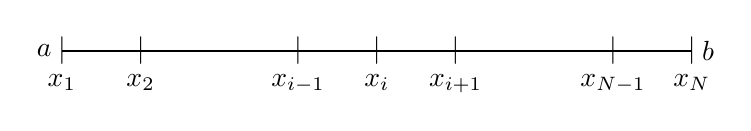
\begin{tikzpicture}[scale=5, nodes={
			execute at begin node= $,
			execute at end node=$}]
		\draw[-, thick]  (-0.8,0) -- (0.8,0)  node[right] {b};
		\foreach \x/\xpar/\xtext in { 
			-0.8 / | / x_{1},
			-0.6 / | / x_{2},
			-0.2 / | / x_{i-1},
			0    / | / x_{i},
			0.2  / | / x_{i+1},
			0.6  / | / x_{N-1},
			0.8  / | / x_{N}
		}
		\draw[thick] (\x,0pt) node {\xpar}  node[below=5pt] {\xtext};
		\draw[-, thick] (-0.8,0)  node[left]{a} ;
		\end{tikzpicture}
	\end{center}
We will consider Taylor's theorem for $u(x)$ at $x= x + \triangle x$ to find the first order forward difference formula, which gives 
\begin{align}{\label{Eq.2_2_1}}
u(x + \triangle x ) & = u(x) + \triangle x \dfrac{\partial u}{\partial x }(x) + \dfrac{\triangle x^{2}}{2!} \dfrac{\partial^{2} u}{\partial x^{2} }(\xi_{1}), \quad \text{where} \hspace{0.15cm} \xi_{1} \in (x , x + \triangle x).
\end{align}
Solving for $\dfrac{\partial u}{\partial x }(x) $
\begin{align} {\label{Eq.2_2_2}}
\dfrac{\partial u}{\partial x }(x) = \dfrac{u(x + \triangle x ) - u(x)}{\triangle x} -  \dfrac{\triangle x}{2} \dfrac{\partial^{2} u}{\partial x^{2} }(\xi_{1}).
\end{align}
Letting $x_{i}=x$, and $x_{i+1} = x+ \triangle x$ in $(\ref{Eq.2_2_2})$ for each $i = 1,2,\dots,N-1$. For notational convenience, we denote $u_{i} =u(x_{i}) $ to get
\begin{align}{\label{Eq.2_2_3}}
\dfrac{\partial u}{\partial x }\bigg|_{i} = \dfrac{u_{i+1}- u_{i}}{\triangle x} -  \dfrac{\triangle x}{2} \dfrac{\partial^{2} u}{\partial x^{2} }(\xi_{1}).
\end{align}
Using big $\mathcal{O}$ notation, (\ref{Eq.2_2_3}) can be written
\begin{align} {\label{Eq.2_2_4}}
\fbox{ $ \displaystyle \dfrac{\partial u}{\partial x }\bigg|_{i} = \dfrac{u_{i+1} - u_{i}}{\triangle x} + \mathcal{O}(\triangle x),\quad i =\overline{1,N-1}.$}
\end{align}
Equation (\ref{Eq.2_2_4}) is called the forward difference formula for $ \dfrac{\partial u}{\partial x }$ at $x = x_{i}$.
%%%%%%%%%%%%%%%%%%%%%%%%%%%%%%%%%%%%%%%%%%%%%%%%%%%%%%%%%%%%%%%%%%%%%%%%%%%%%
\subsection*{In two dimensions}
Let  $\hspace{5cm} u: \mathbb{R}^{2} \longrightarrow \mathbb{R}$
\par
$ \hspace{5.2cm} (x,y) \longmapsto u(x,y)$
\\
be two dimensional function.
\begin{center}
	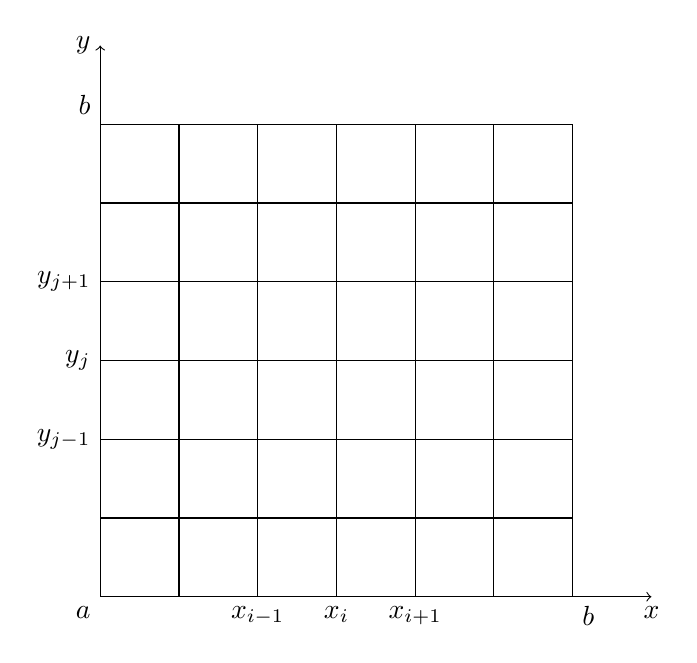
\begin{tikzpicture}[scale=1.0]
	% horizontal axis
	\draw[->] (0,0) -- (7,0) node[anchor=north] {$x$};
	% vertical axis
	\draw[->] (0,0) -- (0,7) node[anchor=east] {$y$};
	% ranges
	\draw (0, 0) grid (6, 6);
	%	\draw (0, 0) rectangle (4, 4);
	\path
	(0, 6) node[above left ] {$b$}
	(6, 0) node[below right] {$b$}
	(0, 0) node[below left] {$a$}
	(2, 0) node[below] {$x_{i-1}$}
	(3, 0) node[below] {$x_{i}$}
	(4, 0) node[below] {$x_{i+1}$}
	(0, 2) node[left] {$y_{j-1}$}
	(0, 3) node[left] {$y_{j}$}
	(0, 4) node[left] {$y_{j+1}$}
	;
	\end{tikzpicture}
\end{center}
We will consider Taylor's theorem  for $u(x,y)$ at $x = x+\triangle x$, which gives
\begin{align*}%{\label{Eq.2_2_5}}
u(x+\triangle x, y) = u(x,y) + \triangle x \dfrac{\partial u}{\partial x}(x, y) + \dfrac{\triangle x^{2}}{2!} \dfrac{\partial^2 u}{\partial x^{2}} (\mu, y),\quad \text{where} \hspace{0.15cm} \mu \in (x, x + \triangle x).
\end{align*}
Solving $\dfrac{\partial u}{\partial x}(x, y)$
\begin{align}{\label{Eq.2_2_6}}
\dfrac{\partial u}{\partial x}(x, y) = \dfrac{u(x+\triangle x ,y ) - u(x,y )  }{\triangle x} -  \dfrac{\triangle x}{2} \dfrac{\partial^2 u}{\partial x^{2}} (\mu, y). 
\end{align}
Letting $(x_{i},y_{j})=(x,y)$, and $(x_{i+1},y_{j})=(x+\triangle x ,y )$ in $(\ref{Eq.2_2_6})$ for each $i = 1,2,\dots,N-1$ and $j = 1,2,\dots,M$. For notational convenience, we denote $u_{i,j}=u(x_{i},y_{j}) $ to get 
\begin{align}{\label{Eq.2_2_7}}
\dfrac{\partial u}{\partial x}\bigg|_{i,j}= \dfrac{u_{i+1,j}- u_{i,j}}{\triangle x} -  \dfrac{\triangle x}{2} \dfrac{\partial^2 u}{\partial x^{2}} (\mu_{i}, y_{j}). 
\end{align}
Using big $\mathcal{O}$ notation, (\ref{Eq.2_2_7}) can be written
\begin{align}{\label{Eq.2_2_8}}
\fbox{ $ \displaystyle \dfrac{\partial u}{\partial x}\bigg|_{i,j}= \dfrac{u_{i+1,j} - u_{i,j}}{\triangle x} + \mathcal{O}(\triangle x),\quad i =\overline{1,N-1}, j=\overline{1,M}.$}
\end{align}
Equation (\ref{Eq.2_2_8}) is called the forward difference formula for $ \dfrac{\partial u}{\partial x }$ at $(x_{i}, y_{j})$.
\\
%%%%%%%%%%%%%%%%%%%%%%%%%%%%%%%%%%%%%%%%%%%%%%%%%%%%%%%%%%%%%%%%%%%%%%%%%%%%
We consider Taylor's theorem for $u(x,y)$ at $y = y + \triangle y$, which gives
\begin{align*}%{\label{Eq.2_2_9}}
u(x, y + \triangle y) = u(x,y) + \triangle y \dfrac{\partial u}{\partial y}(x, y) + \dfrac{\triangle y^{2}}{2!} \dfrac{\partial^2 u}{\partial y^{2}} (x, \eta),\quad \text{where} \hspace{0.15cm} \eta \in (y, y + \triangle y).
\end{align*}
Solving $\dfrac{\partial u}{\partial y}(x, y)$
\begin{align}{\label{Eq.2_2_10}}
\dfrac{\partial u}{\partial y}(x, y) = \dfrac{u(x ,y + \triangle y ) - u(x,y )  }{\triangle y} -  \dfrac{\triangle y}{2} \dfrac{\partial^2 u}{\partial y^{2}} (x, \eta). 
\end{align}
Letting $(x_{i},y_{j})=(x,y)$, and $(x_{i},y_{j+1})=(x ,y+\triangle y )$ in $(\ref{Eq.2_2_10})$ for each $i = 1,2,\dots,N-1$ and $j = 1,2,\dots,M$. For notational convenience, we denote $u_{i,j}=u(x_{i},y_{j}) $ to get 
\begin{align}{\label{Eq.2_2_11}}
\dfrac{\partial u}{\partial y}\bigg|_{i,j} = \dfrac{u_{i,j+1} - u_{i,j}}{\triangle y} -  \dfrac{\triangle y}{2} \dfrac{\partial^2 u}{\partial y^{2}} (x_{i}, \eta_{j}).
\end{align}
Using big $\mathcal{O}$ notation, (\ref{Eq.2_2_11}) can be written
\begin{align}{\label{Eq.2_2_12}}
\fbox{ $ \displaystyle \dfrac{\partial u}{\partial y}\bigg|_{i,j} = \dfrac{u_{i,j+1} - u_{i,j}}{\triangle y} + \mathcal{O}(\triangle y), \quad i =\overline{1,N-1}, j=\overline{1,M}.$}
\end{align}
Equation (\ref{Eq.2_2_12}) is called the forward difference formula for $ \dfrac{\partial u}{\partial y }$ at $(x_{i}, y_{j})$.
%%%%%%%%%%%%%%%%%%%%%%%%%%%%%%%%%%%%%%%%%%%%%%%%%%%%%%%%%%%%%%%%%%%%%%%%%%%%%
\section{First order backward difference}
\subsection*{In one dimension}
Let  $\hspace{5cm} u: \mathbb{R} \longrightarrow \mathbb{R}$
\par
$ \hspace{5.8cm} x \longmapsto u(x)$
\\ 
be one dimensional function.
\\
The discretization of the interval $[a, b]$ into $N$ points is given as
\begin{center}
	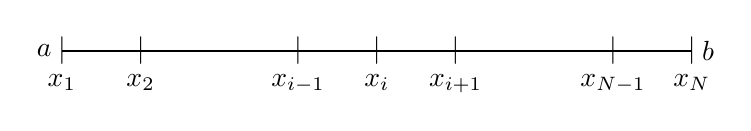
\begin{tikzpicture}[scale=5, nodes={
		execute at begin node= $,
		execute at end node=$}]
	
	\draw[-, thick]  (-0.8,0) -- (0.8,0)  node[right] {b};
	\foreach \x/\xpar/\xtext in { 
		-0.8 / | / x_{1},
		-0.6 / | / x_{2},
		-0.2 / | / x_{i-1},
		0    / | / x_{i},
		0.2  / | / x_{i+1},
		0.6  / | / x_{N-1},
		0.8  / | / x_{N}
	}
	\draw[thick] (\x,0pt) node {\xpar}  node[below=5pt] {\xtext};
	\draw[-, thick] (-0.8,0)  node[left]{a} ;
	\end{tikzpicture}
\end{center}
We will consider Taylor's theorem for $u(x)$ at $x= x - \triangle x$ to find the first order backward difference formula, which gives 
\begin{align*} %{\label{Eq.2_3_1}}
u(x - \triangle x ) = u(x) - \triangle x \dfrac{\partial u}{\partial x }(x) + \dfrac{\triangle x^{2}}{2!} \dfrac{\partial^{2} u}{\partial x^{2} }(\xi_{2}), \quad \text{where} \hspace{0.15cm} \xi_{2} \in (x - \triangle x , x ).
\end{align*}
Solving for $\dfrac{\partial u}{\partial x }(x) $
\begin{align} {\label{Eq.2_3_2}}
\dfrac{\partial u}{\partial x }(x) = \dfrac{ u(x) - u(x - \triangle x ) }{\triangle x} +  \dfrac{\triangle x}{2} \dfrac{\partial^{2} u}{\partial x^{2} }(\xi_{2}).
\end{align}
Letting $x_{i}=x$, and $x_{i-1} = x- \triangle x$ in $(\ref{Eq.2_3_2})$ for each $i = 2,3,\dots,N$. For notational convenience, we denote $u_{i}=u(x_{i})$ to get
\begin{align}{\label{Eq.2_3_3}}
\dfrac{\partial u}{\partial x }\bigg|_{i} = \dfrac{ u_{i}  - u_{i-1}}{\triangle x} +  \dfrac{\triangle x}{2} \dfrac{\partial^{2} u}{\partial x^{2} }(\xi_{2}).
\end{align}
Using big $\mathcal{O}$ notation, (\ref{Eq.2_3_3}) can be written
\begin{align}{\label{Eq.2_3_4}}
\fbox{ $ \displaystyle \dfrac{\partial u}{\partial x }\bigg|_{i}  = \dfrac{u_{i}  - u_{i-1}}{\triangle x} + \mathcal{O}(\triangle x),\quad i =\overline{2,N}.$}
\end{align}
Equation (\ref{Eq.2_3_4}) is called the backward difference formula for $\dfrac{\partial u}{\partial x }$ at $x=x_{i}$.
\\
%%%%%%%%%%%%%%%%%%%%%%%%%%%%%%%%%%%%%%%%%%%%%%%%%%%%%%%%%%%%%%%%%%%%%%%%%%%%%%
\subsection*{In two dimensions}
Let  $\hspace{5cm} u: \mathbb{R}^{2} \longrightarrow \mathbb{R}$
\par
$ \hspace{5.2cm} (x,y) \longmapsto u(x,y)$
\\
be two dimensional function.
\begin{center}
	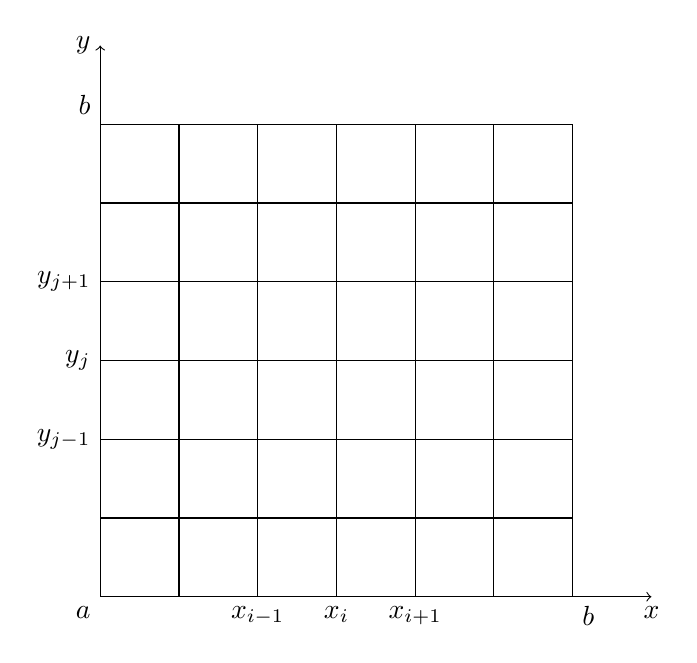
\begin{tikzpicture}[scale=1.0]
	% horizontal axis
	\draw[->] (0,0) -- (7,0) node[anchor=north] {$x$};
	% vertical axis
	\draw[->] (0,0) -- (0,7) node[anchor=east] {$y$};
	% ranges
	\draw (0, 0) grid (6, 6);
	%	\draw (0, 0) rectangle (4, 4);
	\path
	(0, 6) node[above left ] {$b$}
	(6, 0) node[below right] {$b$}
	(0, 0) node[below left] {$a$}
	(2, 0) node[below] {$x_{i-1}$}
	(3, 0) node[below] {$x_{i}$}
	(4, 0) node[below] {$x_{i+1}$}
	(0, 2) node[left] {$y_{j-1}$}
	(0, 3) node[left] {$y_{j}$}
	(0, 4) node[left] {$y_{j+1}$}
	;
	\end{tikzpicture}
\end{center}
Consider Taylor's theorem for $u(x,y)$ at $x= x-\triangle x$, one has
\begin{align*}%{\label{Eq.2_3_5}}
u(x-\triangle x, y) = u(x,y) - \triangle x \dfrac{\partial u}{\partial x}(x, y) + \dfrac{\triangle x^{2}}{2!} \dfrac{\partial^2 u}{\partial x^{2}} (\mu, y), \quad \text{where} \hspace{0.15cm} \mu \in (x - \triangle x, x).
\end{align*}
Solving $\dfrac{\partial u}{\partial x}(x, y)$
\begin{align}{\label{Eq.2_3_6}}
\dfrac{\partial u}{\partial x}(x, y) = \dfrac{u(x,y ) - u(x-\triangle x ,y )  }{\triangle x} +  \dfrac{\triangle x}{2} \dfrac{\partial^2 u}{\partial x^{2}} (\mu, y). 
\end{align}
Letting $(x_{i},y_{j})=(x,y)$, and $(x_{i-1},y_{j})=(x-\triangle x ,y )$  in $(\ref{Eq.2_3_6})$ for each $i = 2,3,\dots,N$ and $j = 1,2,\dots,M$. For notational convenience, we denote $u_{i,j}=u(x_{i},y_{j}) $ to get
\begin{align}{\label{Eq.2_3_7}}
\dfrac{\partial u}{\partial x}\bigg|_{i,j}= \dfrac{ u_{i,j} - u_{i-1,j} }{\triangle x} +  \dfrac{\triangle x}{2} \dfrac{\partial^2 u}{\partial x^{2}} (\mu_{i}, y_{j}). 
\end{align}
Using big $\mathcal{O}$ notation, (\ref{Eq.2_3_7}) can be written
\begin{align}{\label{Eq.2_3_8}}
\fbox{ $ \displaystyle \dfrac{\partial u}{\partial x}\bigg|_{i,j}= \dfrac{ u_{i,j} - u_{i-1,j}}{\triangle x} + \mathcal{O}(\triangle x),\quad i =\overline{2,N}, j=\overline{1,M}. $}
\end{align}
Equation (\ref{Eq.2_3_8}) is called the backward difference formula for $\dfrac{\partial u}{\partial x }$ at $(x_{i}, y_{j})$.
\\
%%%%%%%%%%%%%%%%%%%%%%%%%%%%%%%%%%%%%%%%%%%%%%%%%%%%%%%%%%%%%%%%%%%%%%%%%%%
Consider Taylor's theorem for $u(x,y)$ at $y= y - \triangle y$
\begin{align*}%{\label{Eq.2_3_9}}
u(x, y - \triangle y) = u(x,y) - \triangle y \dfrac{\partial u}{\partial y}(x, y) + \dfrac{\triangle y^{2}}{2!} \dfrac{\partial^2 u}{\partial y^{2}} (x, \eta), \quad \text{where} \hspace{0.15cm}\eta \in (y - \triangle y, y).
\end{align*}
Solving $\dfrac{\partial u}{\partial y}(x, y)$
\begin{align}{\label{Eq.2_3_10}}
\dfrac{\partial u}{\partial y}(x, y) = \dfrac{ u(x,y ) - u(x ,y - \triangle y )  }{\triangle y} +  \dfrac{\triangle y}{2} \dfrac{\partial^2 u}{\partial y^{2}} (x, \eta). 
\end{align}
Letting $(x_{i},y_{j})=(x,y)$, and $(x_{i},y_{j-1})=(x,y -\triangle y )$  in $(\ref{Eq.2_3_10})$ for each $i = 1,2,\dots,N$ and $j = 2,3,\dots,M$. For notational convenience, we denote $u_{i,j}=u(x_{i},y_{j}) $ to get
\begin{align}{\label{Eq.2_3_11}}
\dfrac{\partial u}{\partial y}\bigg|_{i,j} = \dfrac{ u_{i,j} - u_{i,j-1}}{\triangle y} +  \dfrac{\triangle y}{2} \dfrac{\partial^2 u}{\partial y^{2}} (x_{i}, \eta_{j}).
\end{align}
Using big $\mathcal{O}$ notation, (\ref{Eq.2_3_11}) can be written
\begin{align}{\label{Eq.2_3_12}}
\fbox{ $ \displaystyle \dfrac{\partial u}{\partial y}\bigg|_{i,j} = \dfrac{ u_{i,j} - u_{i,j-1}}{\triangle y}  + \mathcal{O}(\triangle y),\quad i =\overline{1,N}, j=\overline{2,M}. $}
\end{align}
%for $i = 1,2,\dots,N$ and $j = 2,3,\dots,M$.
%\\
Equation (\ref{Eq.2_3_12}) is called the backward difference formula for $\dfrac{\partial u}{\partial y }$ at $(x_{i}, y_{j})$.
\\
%%%%%%%%%%%%%%%%%%%%%%%%%%%%%%%%%%%%%%%%%%%%%%%%%%%%%%%%%%%%%%%%%%%%%%%%%%%%%%
\section{First order central difference}
\subsection*{In one dimension}
Let $\hspace{5cm} u:\mathbb{R} \longrightarrow \mathbb{R}$
\par
$ \hspace{5.8cm} x \longmapsto u(x)$
\\
be one dimensional function.
\\
The discretization of the interval $[a, b]$ into $N$ points is given as
\begin{center}
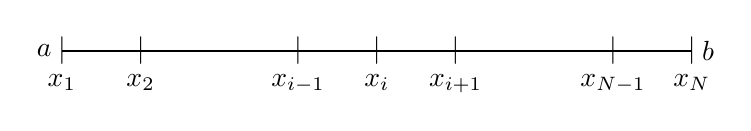
\begin{tikzpicture}[scale=5, nodes={
	execute at begin node= $,
	execute at end node=$}]

\draw[-, thick]  (-0.8,0) -- (0.8,0)  node[right] {b};
\foreach \x/\xpar/\xtext in { 
	-0.8 / | / x_{1},
	-0.6 / | / x_{2},
	-0.2 / | / x_{i-1},
	0    / | / x_{i},
	0.2  / | / x_{i+1},
	0.6  / | / x_{N-1},
	0.8  / | / x_{N}
}
\draw[thick] (\x,0pt) node {\xpar}  node[below=5pt] {\xtext};
\draw[-, thick] (-0.8,0)  node[left]{a} ;
\end{tikzpicture}
\end{center}
Consider Taylor's theorem for $u(x)$ at $x=x + \triangle x $ and $x = x - \triangle x $ to obtain
\begin{align}{\label{Eq.2_4_1}}
u(x + \triangle x ) = u(x) + \triangle x \dfrac{\partial u}{\partial x }(x) + \dfrac{\triangle x^{2}}{2!} \dfrac{\partial^{2} u}{\partial x^{2} }(x) + \dfrac{\triangle x^{3}}{3!} \dfrac{\partial^{3} u}{\partial x^{3} }(\xi_{1}),
\end{align}
where $ \xi_{1} \in (x , x + \triangle x)$.
\begin{align}{\label{Eq.2_4_2}}
u(x - \triangle x ) = u(x) - \triangle x \dfrac{\partial u}{\partial x }(x) + \dfrac{\triangle x^{2}}{2!} \dfrac{\partial^{2} u}{\partial x^{2} }(x) - \dfrac{\triangle x^{3}}{3!} \dfrac{\partial^{3} u}{\partial x^{3} }(\xi_{2}),
\end{align}
where $ \xi_{2} \in ( x - \triangle x, x )$.
\\
We subtract (\ref{Eq.2_4_1}) from (\ref{Eq.2_4_2}) to obtain
\begin{align} {\label{Eq.2_4_3}}
u(x + \triangle x ) - u(x - \triangle x ) =  2 \triangle x \dfrac{\partial u}{\partial x }(x) +  \dfrac{\triangle x^{3}}{3!} \bigg[ \dfrac{\partial^{3} u}{\partial x^{3} }(\xi_{1}) + \dfrac{\partial^{3} u}{\partial x^{3} }(\xi_{2}) \bigg].
\end{align}
The Intermediate Value Theorem is used to deduce that for some number $\xi$, where $\xi_{1} < \xi < \xi_{2}$, (\ref{Eq.2_4_3}) becomes
\begin{align} %{\label{Eq.2_4_4}}
u(x + \triangle x ) - u(x - \triangle x ) =  2 \triangle x \dfrac{\partial u}{\partial x }(x) +  \dfrac{\triangle x^{3}}{3}  \dfrac{\partial^{3} u}{\partial x^{3} }(\xi).
\end{align}
Solving for $\dfrac{\partial u}{\partial x }(x) $
\begin{align} {\label{Eq.2_4_5}}
\dfrac{\partial u}{\partial x }(x) = \dfrac{u(x + \triangle x ) - u(x - \triangle x )}{2 \triangle x } -  \dfrac{\triangle x^{2}}{6} \dfrac{\partial^{3} u}{\partial x^{3} }(\xi).
\end{align}
Letting $x_{i+1} = x+ \triangle x$, and $x_{i-1} = x- \triangle x$ in $(\ref{Eq.2_4_5})$ for each $i = 2,3,\dots,N-1$. For notational convenience, we denote $u_{i}= u(x_{i})$ to get
\begin{align}{\label{Eq.2_4_6}}
\dfrac{\partial u}{\partial x }\bigg|_{i}= \dfrac{ u_{i+1}  - u_{i-1}}{2 \triangle x}  -  \dfrac{\triangle x^{2}}{6} \dfrac{\partial^{3} u}{\partial x^{3} }(\xi).
\end{align}
Using big $\mathcal{O}$ notation, (\ref{Eq.2_4_6}) can be written
\begin{align}{\label{Eq.2_4_7}}
\fbox{ $ \displaystyle \dfrac{\partial u}{\partial x }\bigg|_{i} = \dfrac{u_{i+1} - u_{i-1} }{2\triangle x} + \mathcal{O}(\triangle x^{2}),\quad i =\overline{2,N-1}.$}
\end{align}
Equation (\ref{Eq.2_4_7}) is called the first order central difference formula for $\dfrac{\partial u}{\partial x }$ at $x = x_{i}$.
%%%%%%%%%%%%%%%%%%%%%%%%%%%%%%%%%%%%%%%%%%%%%%%%%%%%%%%%%%%%%%%%%%%%%%%%%%%%%%
\subsection*{In two dimensions}
Let $\hspace{5cm} u: \mathbb{R}^{2} \longrightarrow \mathbb{R}$
\par
$ \hspace{5.2cm} (x,y) \longmapsto u(x,y)$
\\
be two dimensional function.
\begin{center}
	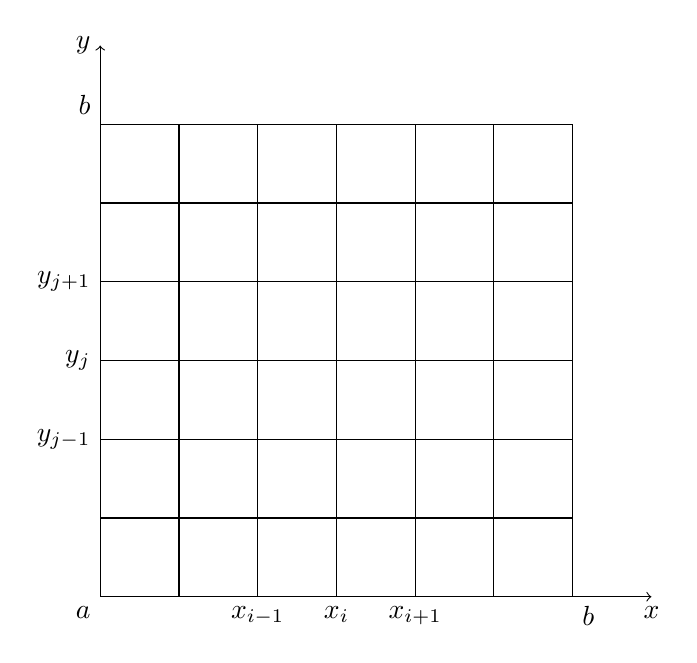
\begin{tikzpicture}[scale=1.0]
	% horizontal axis
	\draw[->] (0,0) -- (7,0) node[anchor=north] {$x$};
	% vertical axis
	\draw[->] (0,0) -- (0,7) node[anchor=east] {$y$};
	% ranges
	\draw (0, 0) grid (6, 6);
	%	\draw (0, 0) rectangle (4, 4);
	\path
	(0, 6) node[above left ] {$b$}
	(6, 0) node[below right] {$b$}
	(0, 0) node[below left] {$a$}
	(2, 0) node[below] {$x_{i-1}$}
	(3, 0) node[below] {$x_{i}$}
	(4, 0) node[below] {$x_{i+1}$}
	(0, 2) node[left] {$y_{j-1}$}
	(0, 3) node[left] {$y_{j}$}
	(0, 4) node[left] {$y_{j+1}$}
	;
	\end{tikzpicture}
\end{center}
Consider Taylor's theorem for $u(x,y)$ at $x=x + \triangle x $ and $x = x - \triangle x $ to obtain
\begin{align}{\label{Eq.2_4_8}}
u(x+\triangle x, y) = u(x,y) + \triangle x \dfrac{\partial u}{\partial x}(x, y) + \dfrac{\triangle x^{2}}{2!} \dfrac{\partial^2 u}{\partial x^{2}} (x, y) +  \dfrac{\triangle x^{3}}{3!} \dfrac{\partial^3 u}{\partial x^{3}} (\xi_{1}, y) ,
\end{align}
where $\xi_{1} \in (x, x + \triangle x)$.
\begin{align}{\label{Eq.2_4_9}}
u(x-\triangle x, y) = u(x,y) - \triangle x \dfrac{\partial u}{\partial x}(x, y) + \dfrac{\triangle x^{2}}{2!} \dfrac{\partial^2 u}{\partial x^{2}} (x, y) -  \dfrac{\triangle x^{3}}{3!} \dfrac{\partial^3 u}{\partial x^{3}} (\xi_{2}, y) ,
\end{align}
where $\xi_{2} \in (x - \triangle x, x)$.
\\
We subtract  (\ref{Eq.2_4_8}) from (\ref{Eq.2_4_9}), we get 
\begin{align}{\label{Eq.2_4_10}}
u(x+\triangle x, y) - u(x-\triangle x, y) = 2 \triangle x \dfrac{\partial u}{\partial x}(x, y) + \dfrac{\triangle x^{3}}{3!} \bigg [ \dfrac{\partial^3 u}{\partial x^{3}} (\xi_{1}, y) +    \dfrac{\partial^3 u}{\partial x^{3}} (\xi_{2}, y)  \bigg].
\end{align}
The Intermediate Value Theorem is used to deduce that for some number $\xi$, where $\xi_{1} < \xi < \xi_{2}$, (\ref{Eq.2_4_10}) becomes
\begin{align*}%{\label{Eq.2_4_11}}
u(x+\triangle x, y) - u(x-\triangle x, y) = 2 \triangle x \dfrac{\partial u}{\partial x}(x, y) +  \dfrac{\triangle x^{3}}{3} \dfrac{\partial^3 u}{\partial x^{3}} (\xi, y).
\end{align*}
Solving $\dfrac{\partial u}{\partial x}(x, y) $ 
\begin{align}{\label{Eq.2_4_12}}
\dfrac{\partial u}{\partial x}(x, y) = \dfrac{u(x+\triangle x, y) - u(x-\triangle x, y)}{2 \triangle x } - \dfrac{\triangle x^{2}}{6} \dfrac{\partial^3 u}{\partial x^{3}} (\xi, y).
\end{align}
Letting $(x_{i+1},y_{j})=(x+\triangle x,y)$, and $(x_{i-1},y_{j})=(x-\triangle x ,y )$  in $(\ref{Eq.2_4_12})$ for each $i = 2,3,\dots,N-1$ and $j=1,2,\dots,M$. For notational convenience, we denote $u_{i,j}= u(x_{i},y_{j})$ to get
\begin{align}{\label{Eq.2_4_13}}
\dfrac{\partial u}{\partial x}\bigg|_{i,j} = \dfrac{u_{i+1,j} - u_{i-1,j}}{2 \triangle x } - \dfrac{\triangle x^{2}}{6} \dfrac{\partial^3 u}{\partial x^{3}} (\xi_{i}, y_{j}).
\end{align}
Using big $\mathcal{O}$ notation, (\ref{Eq.2_4_13}) can be written
\begin{align}{\label{Eq.2_4_14}}
\fbox{ $ \displaystyle\dfrac{\partial u}{\partial x}\bigg|_{i,j} = \dfrac{u_{i+1,j} - u_{i-1,j}}{2 \triangle x } + \mathcal{O}(\triangle x^{2}),\quad i =\overline{2,N-1}, j=\overline{1,M}.$}
\end{align}
Equation (\ref{Eq.2_4_14}) is called the first order central difference formula for $\dfrac{\partial u}{\partial x }$ at $(x_{i}, y_{j})$.
\\
%%%%%%%%%%%%%%%%%%%%%%%%%%%%%%%%%%%%%%%%%%%%%%%%%%%%%%%%%%%%%%%%%%%%%%%%%%%%%%
Consider Taylor's theorem for $u(x,y)$ at $y =  y + \triangle y $ and $y = y - \triangle y $ to obtain
\begin{align}{\label{Eq.2_4_15}}
u(x, y + \triangle y) = u(x,y) + \triangle y \dfrac{\partial u}{\partial y}(x, y) + \dfrac{\triangle y^{2}}{2!} \dfrac{\partial^2 u}{\partial y^{2}} (x, y) +  \dfrac{\triangle y^{3}}{3!} \dfrac{\partial^3 u}{\partial y^{3}} (x, \xi_{1}) ,
\end{align}
where $\xi_{1} \in (y, y + \triangle y)$.
\begin{align}{\label{Eq.2_4_16}}
u(x, y - \triangle y) = u(x,y) - \triangle y \dfrac{\partial u}{\partial y}(x, y) + \dfrac{\triangle y^{2}}{2!} \dfrac{\partial^2 u}{\partial y^{2}} (x, y) -  \dfrac{\triangle y^{3}}{3!} \dfrac{\partial^3 u}{\partial y^{3}} (x,\xi_{2}) ,
\end{align}
where $\xi_{2} \in (y - \triangle y, y)$.
\\
We subtract (\ref{Eq.2_4_15}) from (\ref{Eq.2_4_16}), we get 
\begin{align}{\label{Eq.2_4_17}}
u(x, y + \triangle y)- u(x, y - \triangle y) = 2 \triangle y \dfrac{\partial u}{\partial y}(x, y) + \dfrac{\triangle y^{3}}{3!} \bigg [ \dfrac{\partial^3 u}{\partial y^{3}} (x,\xi_{1}) +    \dfrac{\partial^3 u}{\partial y^{3}} (x,\xi_{2})  \bigg].
\end{align}
The Intermediate Value Theorem is used to deduce that for some number $\xi$, where $\xi_{1} < \xi < \xi_{2}$, (\ref{Eq.2_4_17}) becomes
\begin{align*}%{\label{Eq.2_4_18}}
u(x, y + \triangle y)- u(x, y - \triangle y) = 2 \triangle y \dfrac{\partial u}{\partial y}(x, y) +  \dfrac{\triangle y^{3}}{3} \dfrac{\partial^3 u}{\partial y^{3}} (x,\xi).
\end{align*}
Solving $\dfrac{\partial u}{\partial y}(x, y) $ 
\begin{align}{\label{Eq.2_4_19}}
\dfrac{\partial u}{\partial y}(x, y) = \dfrac{u(x, y + \triangle y)- u(x, y - \triangle y)}{2 \triangle y } - \dfrac{\triangle y^{2}}{6} \dfrac{\partial^3 u}{\partial y^{3}} (x,\xi).
\end{align}
Letting $(x_{i},y_{j+1})=(x,y+\triangle y)$, and $(x_{i},y_{j-1})=(x,y-\triangle y )$  in $(\ref{Eq.2_4_19})$ for each $i = 1,2,\dots,N$ and $j=2,3,\dots,M-1 $. For notational convenience, we denote $u_{i,j}= u(x_{i},y_{j})$ to get
\begin{align}{\label{Eq.2_4_20}}
\dfrac{\partial u}{\partial y}\bigg|_{i, j} = \dfrac{u_{i,j+1} - u_{i,j-1}}{2 \triangle y } - \dfrac{\triangle y^{2}}{6} \dfrac{\partial^3 u}{\partial y^{3}} (x_{i}, \xi_{j}).
\end{align}
Using big $\mathcal{O}$ notation, (\ref{Eq.2_4_20}) can be written
\begin{align}{\label{Eq.2_4_21}}
\fbox{ $ \displaystyle \dfrac{\partial u}{\partial y}\bigg|_{i, j}  = \dfrac{u_{i,j+1} - u_{i,j-1}}{2 \triangle y } + \mathcal{O}(\triangle y^{2}),\quad i =\overline{1,N}, j=\overline{2,M-1}.$}
\end{align}
Equation (\ref{Eq.2_4_21}) is called the first order central difference formula for $\dfrac{\partial u}{\partial y }$ at $(x_{i}, y_{j})$.
%--------------------------------------------------------------------------------------------------
\section{Second order central difference}
\subsection*{In one dimension}
Let $\hspace{5cm} u: \mathbb{R} \longrightarrow \mathbb{R}$
\par
$ \hspace{5.8cm} x \longmapsto u(x)$
\\
be one dimensional function.
\\
The discretization of the interval $[a, b]$ into $N$ points is given as
\begin{center}
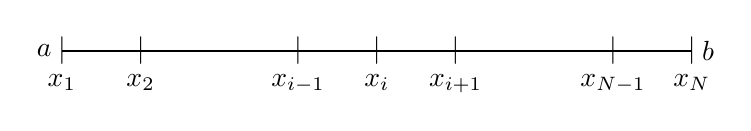
\begin{tikzpicture}[scale=5, nodes={
	execute at begin node= $,
	execute at end node=$}]

\draw[-, thick]  (-0.8,0) -- (0.8,0)  node[right] {b};
\foreach \x/\xpar/\xtext in { 
	-0.8 / | / x_{1},
	-0.6 / | / x_{2},
	-0.2 / | / x_{i-1},
	0    / | / x_{i},
	0.2  / | / x_{i+1},
	0.6  / | / x_{N-1},
	0.8  / | / x_{N}
}
\draw[thick] (\x,0pt) node {\xpar}  node[below=5pt] {\xtext};
\draw[-, thick] (-0.8,0)  node[left]{a} ;
\end{tikzpicture}
\end{center}
Consider Taylor's theorem for $u(x)$ at $x=x + \triangle x $ and $x = x - \triangle x $ to obtain 
\begin{align}{\label{Eq.2_5_1}}
u(x + \triangle x ) = u(x) + \triangle x \dfrac{\partial u}{\partial x }(x) + \dfrac{\triangle x^{2}}{2!} \dfrac{\partial^{2} u}{\partial x^{2} }(x) + \dfrac{\triangle x^{3}}{3!} \dfrac{\partial^{3} u}{\partial x^{3} }(x) + \dfrac{\triangle x^{4}}{4!} \dfrac{\partial^{4} u}{\partial x^{4} }(\xi_{1}),
\end{align}
where $ \xi_{1} \in (x , x + \triangle x)$.
\begin{align}{\label{Eq.2_5_2}}
u(x - \triangle x ) = u(x) - \triangle x \dfrac{\partial u}{\partial x }(x) + \dfrac{\triangle x^{2}}{2!} \dfrac{\partial^{2} u}{\partial x^{2} }(x) - \dfrac{\triangle x^{3}}{3!} \dfrac{\partial^{3} u}{\partial x^{3} }(x) + \dfrac{\triangle x^{4}}{4!} \dfrac{\partial^{4} u}{\partial x^{4} }(\xi_{2}),
\end{align}
where $ \xi_{2} \in (x - \triangle x, x)$.
\\
Adding (\ref{Eq.2_5_1}) to (\ref{Eq.2_5_2}), one gets
\begin{align} {\label{Eq.2_5_3}}
u(x + \triangle x ) + u(x - \triangle x ) = 2u(x) + \triangle x^{2} \dfrac{\partial^{2} u}{\partial x^{2} }(x) +  \dfrac{\triangle x^{4}}{4!} \bigg [  \dfrac{\partial^{4} u}{\partial x^{4} }(\xi_{1}) + \dfrac{\partial^{4} u}{\partial x^{4} }(\xi_{2}) \bigg ],
\end{align}
The Intermediate Value Theorem is used to deduce that for some number $\xi$, where $\xi_{1} < \xi < \xi_{2}$, (\ref{Eq.2_5_3}) becomes
\begin{align*} %{\label{Eq.2_5_4}}
u(x + \triangle x ) + u(x - \triangle x ) = 2u(x) + \triangle x^{2} \dfrac{\partial^{2} u}{\partial x^{2} }(x) +   \dfrac{\triangle x^{4}}{12}  \dfrac{\partial^{4} u}{\partial x^{4} }(\xi),
\end{align*}
Solving for $\dfrac{\partial^{2} u}{\partial x^{2} }(x) $
\begin{align} {\label{Eq.2_5_5}}
\dfrac{\partial^{2} u}{\partial x^{2} }(x)  = \dfrac{u(x + \triangle x ) - 2u(x) + u(x - \triangle x )}{ \triangle x^{2}} -  \dfrac{\triangle x^{2}}{12} \dfrac{\partial^{4} u}{\partial x^{4} }(\xi).
\end{align}
Letting $x_{i+1} = x+ \triangle x$, $x_{i} = x$ and $x_{i-1} = x- \triangle x$ in $(\ref{Eq.2_5_5})$ for each $i = 2,3,\dots,N-1$. For notational convenience, we denote $u_{i}=u(x_{i})$ to get
\begin{align}{\label{Eq.2_5_6}}
\dfrac{\partial^{2} u}{\partial x^{2} }\bigg|_{i}  = \dfrac{u_{i+1} - 2u_{i}+ u_{i-1}}{ \triangle x^{2}} -  \dfrac{\triangle x^{2}}{12} \dfrac{\partial^{4} u}{\partial x^{4} }(\xi).
\end{align}
Using big $\mathcal{O}$ notation, (\ref{Eq.2_5_6}) can be written
\begin{align}{\label{Eq.2_5_7}}
\fbox{ $ \displaystyle \dfrac{\partial^{2} u}{\partial x^{2} }\bigg|_{i}  = \dfrac{u_{i+1}  - 2u_{i} + u_{i-1}}{ \triangle x^{2}} + \mathcal{O}(\triangle x^{2}),\quad i =\overline{2,N-1}. $}
\end{align}
Equation (\ref{Eq.2_5_7}) is called the second order central difference formula for $\dfrac{\partial^{2} u}{\partial x^{2} }$ at $ x =x_{i} $.
%%%%%%%%%%%%%%%%%%%%%%%%%%%%%%%%%%%%%%%%%%%%%%%%%%%%%%%%%%%%%%%%%%%%%%%%%%%%
\subsection*{In two dimensions}
Let  $\hspace{5cm} u: \mathbb{R}^{2} \longrightarrow \mathbb{R}$
\par
$ \hspace{5.2cm} (x,y) \longmapsto u(x,y)$
\\
be two dimensional function.
\begin{center}
	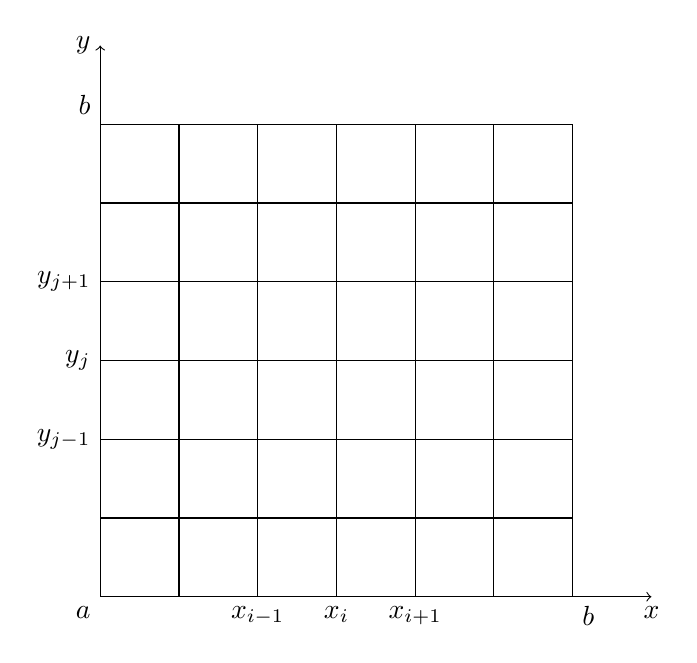
\begin{tikzpicture}[scale=1.0]
	% horizontal axis
	\draw[->] (0,0) -- (7,0) node[anchor=north] {$x$};
	% vertical axis
	\draw[->] (0,0) -- (0,7) node[anchor=east] {$y$};
	% ranges
	\draw (0, 0) grid (6, 6);
	%	\draw (0, 0) rectangle (4, 4);
	\path
	(0, 6) node[above left ] {$b$}
	(6, 0) node[below right] {$b$}
	(0, 0) node[below left] {$a$}
	(2, 0) node[below] {$x_{i-1}$}
	(3, 0) node[below] {$x_{i}$}
	(4, 0) node[below] {$x_{i+1}$}
	(0, 2) node[left] {$y_{j-1}$}
	(0, 3) node[left] {$y_{j}$}
	(0, 4) node[left] {$y_{j+1}$}
	;
	\end{tikzpicture}
\end{center}
Consider Taylor's theorem for $u(x, y)$ at $x=x + \triangle x $ and $x = x - \triangle x $ to obtain
\begin{align}{\label{Eq.2_5_8}}
\begin{split}
u(x+\triangle x, y) = u(x,y) + \triangle x \dfrac{\partial u}{\partial x}(x, y) & + \dfrac{\triangle x^{2}}{2!} \dfrac{\partial^2 u}{\partial x^{2}} (x, y)
\\
& +  \dfrac{\triangle x^{3}}{3!} \dfrac{\partial^3 u}{\partial x^{3}} (x, y)+ \dfrac{\triangle x^{4}}{4!} \dfrac{\partial^4 u}{\partial x^{4}} (\xi_{1}, y),
\end{split}
\end{align}
where $\xi_{1} \in (x, x + \triangle x)$.
\begin{align}{\label{Eq.2_5_9}}
\begin{split}
u(x-\triangle x, y) = u(x,y) - \triangle x \dfrac{\partial u}{\partial x}(x, y) &+ \dfrac{\triangle x^{2}}{2!} \dfrac{\partial^2 u}{\partial x^{2}} (x, y)
\\
& -  \dfrac{\triangle x^{3}}{3!} \dfrac{\partial^3 u}{\partial x^{3}} (x, y) + \dfrac{\triangle x^{4}}{4!} \dfrac{\partial^4 u}{\partial x^{4}} (\xi_{2}, y),
\end{split}
\end{align}
where $\xi_{2} \in (x - \triangle x, x)$.
\\
Adding (\ref{Eq.2_5_8}) to (\ref{Eq.2_5_9}), one gets 
\begin{align}{\label{Eq.2_5_10}}
\begin{split}
u(x+\triangle x, y) + u(x-\triangle x, y) = 2 u(x, y) & +  \triangle x^{2} \dfrac{\partial^2 u}{\partial x^{2}} (x, y) 
\\
&+ \dfrac{\triangle x^{4}}{4!} \bigg [ \dfrac{\partial^4 u}{\partial x^{4}} (\xi_{1}, y)
+ \dfrac{\partial^4 u}{\partial x^{4}} (\xi_{2}, y)  \bigg].
\end{split}
\end{align}
The Intermediate Value Theorem is used to deduce that for some number $\xi$, where $\xi_{1} < \xi < \xi_{2}$, (\ref{Eq.2_5_10}) becomes
\begin{align*}%{\label{Eq.2_5_11}}
u(x+\triangle x, y) + u(x-\triangle x, y) = 2 u(x, y) + \triangle x^{2} \dfrac{\partial^2 u}{\partial x^{2}} (x, y) +  \dfrac{\triangle x^{4}}{12} \dfrac{\partial^4 u}{\partial x^{4}} (\xi, y)
\end{align*}
Solving $ \dfrac{\partial^2 u}{\partial x^{2}} (x, y) $ 
\begin{align}{\label{Eq.2_5_12}}
\dfrac{\partial^2 u}{\partial x^{2}} (x, y) = \dfrac{u(x+\triangle x, y) -  2 u(x, y) + u(x-\triangle x, y)}{\triangle x^{2}} -  \dfrac{\triangle x^{2}}{12} \dfrac{\partial^4 u}{\partial x^{4}} (\xi, y)
\end{align}
Letting $(x_{i+1},y_{j}) = (x+ \triangle x,y)$, $(x_{i},y_{j}) = (x,y)$ and $(x_{i-1},y_{j}) = (x- \triangle x,y)$ in $(\ref{Eq.2_5_12})$ for each $i = 2,3,\dots,N-1$ and $j=1,2,\dots,M$. For notational convenience, we denote $u_{i,j}=u(x_{i},y_{j})$ to get
\begin{align}{\label{Eq.2_5_13}}
\dfrac{\partial^2 u}{\partial x^{2}}\bigg|_{i,j} = \dfrac{u_{i+1,j}-  2 u_{i,j} + u_{i-1,j}}{\triangle x^{2}} -  \dfrac{\triangle x^{2}}{12} \dfrac{\partial^4 u}{\partial x^{4}} (\xi_{i}, y_{j})
\end{align}
Using big $\mathcal{O}$ notation, (\ref{Eq.2_5_13}) can be written
\begin{align}{\label{Eq.2_5_14}}
\fbox{ $ \displaystyle \dfrac{\partial^2 u}{\partial x^{2}}\bigg|_{i,j} = \dfrac{u_{i+1,j}-  2 u_{i,j} + u_{i-1,j}}{\triangle x^{2}} + \mathcal{O}(\triangle x^{2}),\quad i =\overline{2,N-1}, j=\overline{1,M}.$}
\end{align}
Equation (\ref{Eq.2_5_14}) is called the second-order central difference formula for $\dfrac{\partial^{2} u}{\partial x^{2}}$ at $(x_{i}, y_{j})$.
\\
%%%%%%%%%%%%%%%%%%%%%%%%%%%%%%%%%%%%%%%%%%%%%%%%%%%%%%%%%%%%%%%%%%%%%%%%%%%%%%%%%
Consider Taylor's theorem for $u(x, y )$ at $y=y + \triangle y $ and $y = y - \triangle y $ to obtain
\begin{align}{\label{Eq.2_5_15}}
\begin{split}
u(x, y + \triangle y) = u(x,y) + \triangle y \dfrac{\partial u}{\partial y}(x, y) & + \dfrac{\triangle y^{2}}{2!} \dfrac{\partial^2 u}{\partial y^{2}} (x, y) 
\\
& +  \dfrac{\triangle y^{3}}{3!} \dfrac{\partial^3 u}{\partial y^{3}} (x, y) + \dfrac{\triangle y^{4}}{4!} \dfrac{\partial^4 u}{\partial y^{4}} (x, \xi_{1}),
\end{split}
\end{align}
where $\xi_{1} \in (y, y + \triangle y)$.
\begin{align}{\label{Eq.2_5_16}}
\begin{split}
u(x, y - \triangle y) = u(x,y) - \triangle y \dfrac{\partial u}{\partial y}(x, y) & + \dfrac{\triangle y^{2}}{2!} \dfrac{\partial^2 u}{\partial y^{2}} (x, y) 
\\
& -  \dfrac{\triangle y^{3}}{3!} \dfrac{\partial^3 u}{\partial y^{3}} (x,\xi_{2})  + \dfrac{\triangle y^{4}}{4!} \dfrac{\partial^4 u}{\partial y^{4}} (x, \xi_{2}),
\end{split}
\end{align}
where $\xi_{2} \in (y - \triangle y, y)$.
\\
We add (\ref{Eq.2_5_15}) to (\ref{Eq.2_5_16}), we get 
\begin{align}{\label{Eq.2_5_17}}
\begin{split}
u(x, y + \triangle y)+ u(x, y - \triangle y) = 2 u(x, y) & + \triangle y^{2}\dfrac{\partial^2 u}{\partial y^{2}} (x, y) 
\\
& + \dfrac{\triangle y^{4}}{4!} \bigg [ \dfrac{\partial^4 u}{\partial y^{4}} (x,\xi_{1}) +    \dfrac{\partial^4 u}{\partial y^{4}} (x,\xi_{2})  \bigg].
\end{split}
\end{align}
The Intermediate Value Theorem is used to deduce that for some number $\xi$, where $\xi_{1} < \xi < \xi_{2}$, (\ref{Eq.2_5_17}) becomes
\begin{align*}%{\label{Eq.2_5_18}}
u(x, y + \triangle y)+ u(x, y - \triangle y) = 2 u(x, y) + \triangle y^{2}\dfrac{\partial^2 u}{\partial y^{2}} (x, y) +  \dfrac{\triangle y^{4}}{12} \dfrac{\partial^4 u}{\partial y^{4}} (x,\xi).
\end{align*}
Solving $\dfrac{\partial^2 u}{\partial y^{2}} (x, y) $ 
\begin{align}{\label{Eq.2_5_19}}
\dfrac{\partial^2 u}{\partial y^{2}} (x, y)= \dfrac{u(x, y + \triangle y) - 2 u(x, y) + u(x, y - \triangle y)}{ \triangle  y^{2} } -  \dfrac{\triangle y^{2}}{12} \dfrac{\partial^4 u}{\partial y^{4}} (x,\xi).
\end{align}
Letting $(x_{i},y_{i+1}) = (x,y+ \triangle y)$, $(x_{i},y_{j}) = (x,y)$ and $(x, y_{i-1}) = (x,y- \triangle y)$ in $(\ref{Eq.2_5_19})$ for each $i=1,2,\dots,N$ and $j = 2,3,\dots,M-1$. For notational convenience, we denote $u_{i,j}= u(x_{i},y_{j})$ to get
\begin{align}{\label{Eq.2_5_20}}
\dfrac{\partial^2 u}{\partial y^{2}}\bigg|_{i,j}= \dfrac{u_{i,j+1} - 2 u_{i,j}+ u_{i,j-1} }{ \triangle  y^{2} } -  \dfrac{\triangle y^{2}}{12} \dfrac{\partial^4 u}{\partial y^{4}} (x_{i},\xi_{j}).
\end{align}
Using big $\mathcal{O}$ notation, (\ref{Eq.2_5_20}) can be written
\begin{align}{\label{Eq.2_5_21}}
\fbox{ $ \displaystyle \dfrac{\partial^2 u}{\partial y^{2}}\bigg|_{i,j}= \dfrac{u_{i,j+1} - 2 u_{i,j}+ u_{i,j-1} }{ \triangle  y^{2} } + \mathcal{O}(\triangle y^{2}),\quad i =\overline{1,N}, j=\overline{2,M-1}.$}
\end{align}
Equation (\ref{Eq.2_5_21}) is called the second order central difference formula for $\dfrac{\partial^{2} u}{\partial y^{2} } $ at $(x_{i}, y_{j})$.